\documentclass[final,onefignum,onetabnum]{siamart190516}
\usepackage[utf8]{inputenc}
\usepackage{geometry, graphicx,wrapfig}
\usepackage{enumerate}
\usepackage{amsmath,amssymb,amsfonts,bm}%,amsthm}
\usepackage{xcolor} %just for visible comments.
\usepackage[linesnumbered,ruled,vlined,algo2e]{algorithm2e}
\usepackage[toc,page]{appendix}
\usepackage{makecell}
\usepackage{cleveref}
\usepackage{pdfpages}

% New theorems and commands
\newtheorem{assump}[theorem]{MP Setting}
\newcommand\mycommfont[1]{\ttfamily\textcolor{orange}{#1}}
\newcommand{\R}{\mathbb{R}}
\newcommand{\F}{\mathbb{F}}
\newcommand{\dd}{\delta}
\newcommand{\tth}{\theta}
\newcommand{\bb}[1]{\mathbf{#1}}
\newcommand{\fl}{\mathrm{fl}}
\newcommand{\cO}{\mathcal{O}}
\newcommand{\red}[1]{\textcolor{red}{#1}}
\begin{document}
\title{Response to Reviewers}
\date{Octobe 1, 2020}
\maketitle
We are grateful to our editor, Laura Grigori, for handling the reviews of our paper, and to both reviewers for their constructive criticisms.

Our response to the reviews is below, and we have appended a diff file at the end that highlights which changes have been made.\\

\noindent{\bf Reviewer \#1}
%{\it I find the reorganization and reframing of the paper to be an improvement. I believe that the work has merit and deserves to be published. However, in my opinion further revision is required before this can be considered. Some of the main issues I find are the use of the term "backward error" and the treatment of the "disparity in precisions". Namely, there must be some constraint on the disparity in precisions in order for the assumption of "full precision" to apply, but this is not stated clearly.}
\begin{enumerate}
    \item {\it line 5: ``lower storage'' $\rightarrow$ ``lower storage cost'' or ``lower storage requirement'' }\\
    {\bf Done.}
    \item {\it line 13: Inconsistent use of ``round off'' and ``round-off'' (see, e.g., line 16) }\\
    {\bf Done.}
    \item {\it line 11: Inconsistent hyphenation, e.g. ``low precision'' in line 11 and ``high-precision'' in line 21 }\\
    {\bf Done.}
    \item {\it line 25: What is the ``weight of memory''? ``4x'' versus what? }\\
    {\bf We were referring to the physical weight for application like drones. However, it is not necessary for this sentence and therefore has been removed. }
    \item {\it line 36: ``computed up to 16x than that of fp64''--- do you mean ``16x faster''? }\\
    {\bf Done.}
    \item {\it lines 36-37: ``The existing rounding error analyses are built within ...'' Existing rounding error analyses of what? }\\
    {\bf Done ( added ``of linear algebra routines'').}
    \item {\it line 39: This is the first time that HH QR (or QR factorization at all) is even mentioned. The problem that you are considering should be stated earlier in the text. }\\
    {\bf We have included an additional sentence at the end of the first paragraph of the introduction that mentions the QR factorization.}
    \item {\it lines 43-44: ``... its block variants that partition the columns ... and those that partition the columns'' Is there some typo here? }\\
    {\bf Fixed.}
    \item {\it line 58: What does ``sufficient in performance'' mean? }\\
    {\bf This is now clarified.}
    \item {\it line 137: The ``(j,k)'' in the max should not be a subscript. }\\
    {\bf Done.}
    \item {\it line 144: State here what algorithms 5 and 6 are, since they have not been introduced yet. }\\
    {\bf Done.}
    \item {\it line 145: Define what is meant by ``ad hoc''. }\\
    {\bf We simply mean that MP Setting 2.3 is one we have constructed and there's no hardware that implements it to the best of our knowledge currently.}
    \item {\it line 155: ``is in'' $\rightarrow $ ``in'' }\\
    {\bf Done.}
    \item {\it line 157: There is no ``Assumption 2.3''. I assume you meant ``MP Setting 2.3''. }\\
    {\bf Done.}
    \item {\it line 157-160: It might help to give a verbal summary of this, i.e., ``When two fp16 numbers are multiplied and stored in fp32, there is no roundoff error''. }\\
    {\bf Done.}
    \item {\it line 168: The concept of ``full precision'' needs some additional constraint. By my understanding, this ``full precision'' argument only applies when $u^{(h)} \leq (u^{(l)})^2$. If so, then this constraint should be stated explicitly. This further contrains the values that the ``disparity in the precisions'' $M_{l,h}$ can have (line 192). It would be good to state these bounds on $M_{l,h}$. }\\
    {\bf We realize the impreciseness of ``full precision'' in general terms. We first encountered this term in the NVIDIA's description of the TensorCore technology (see \cite{Nvidia2017}), and determined that for IEEE fp16, fp32, and fp64, this means exact product. We have changed the wording the definition of MP Setting 2.3 to reflect this but still leave the analysis that shows that a full precision product of 2 fp16 numbers is exact when represented in fp32. Furthermore, the constraint on $M_{l,h}$ if $u^{(h)} \leq (u^{(l)})^2$ is required certainly improves the accuracy of the mixed precision arithmetic, and much or our analysis is inspired by TC bFMAs. However, we are trying to leave the analysis general so that other combinations of floating point numbers can be considered as well.}
    \item {\it line 288: extra plus sign in ``2(m+2)+''. }\\
    {\bf Done.}
    \item {\it line 288-289: ``swept that minor difference between under'' Some typo/extra word here. }\\
    {\bf Done.}
    \item {\it Lemma 3.2: This use of ``$\delta$'' is different than before, and different than that defined in Table 1. I would use some other symbol here. }\\
    {\bf Done. ($\tau$)}
    \item {\it line 341: I am confused as to where the ``r'' exponent is coming from. }\\
    {\bf We changed the product in Lemma 3.2 to range from $j=1$ to $r$ (it was previously $n$) to better fit how it is used in the proof of Lemma 3.3. }
    \item {\it line 359 (and throughout the text): It is incorrect to refer to $\|\bb{A}-\hat{\bb{Q}}\hat{\bb{R}}\|$ as a backward error. This is better referred to as the ``residual''. The backward error is the quantity which minimizes the difference $\bb{A}-\hat{\bb{Q}}\hat{\bb{R}}$ over all orthogonal matrices Q. The backward error may be bounded in terms of the loss of orthogonality and the residual. } \\
    {\bf We have added the definition of the backward error that is used in this manuscript in the introductary paragraph of Section 2. While $\|\bb{A}-\hat{\bb{Q}}\hat{\bb{R}}\|$ can be referred to as a residual, we prefer to continue to call it a backward error. }
    \item {\it line 399: ``negligble'' spelling }\\
    {\bf Fixed.}
    \item {\it line 416: Where is $\Delta X_k^{(j)}$ defined? }\\
    {\bf This is now explicitly defined.}
    \item {\it line 441: missing period after displayed equation }\\
    {\bf Added.}
    \item {\it line 494: $2^{(l)}$ should be $2^L$, correct? }\\
    {\bf Yes! Thanks for catching that.}
    \item {\it line 536 (and elsewhere): $m2^{-L}$ would look nicer as $2^{-L}m$ }\\
    {\bf Done.}
    \item {\it line 548: The $\gamma$ notation here is not consistent with the rest of the text (gamma with a superscript in parenthesis is used for different precisions; the superscripts here should just be subscripts) }\\
    {\bf Fixed.}
    \item {\it lines 552-553: This case ..." Ok, but do we really expect this in practice? Say something about this. }\\
    {\bf We have added: ``Note that this likely is not the typical situation in practice.'' }
    \item {\it line 556: `2Ln'' typo }\\
    {\bf We got $2Ln$ from the approximation $L\gamma_{2n}=L\frac{2nu}{1-2nu}\approx 2Lnu$.}
    \item {\it line 684-685: "Therefore, the loss ..." But again, there is some constraint on the disparity between precisions in order for the "full precision" assumption to apply, correct? }\\
    {\bf Yes, but now we have added an additional assumption that there is enough disparity such that full precision products are exact indeed. We have added further analysis to this paragraph to clarify how this can be used in practice.  }
    %\red{If we address this, we should go back to defining MP Setting 2.3 with full precision and making a comment about how that affects $M_{l,h}$. Should we do this? Or we could say some blanket statement earlier on about how the disparity we assumed to be large and therefore $M_{l,h}$ is sufficiently large? Also this is brought up in section 4.1, so need to do something about this as well.}
    \item {\it line 694-695: Why is the exact algorithm for mixed precision TSQR omitted? }\\
    {\bf Given the length of the manuscript, we omitted this since the procedure of adding mixed precision to TSQR is similar to how we added mixed precision to BQR (which had been explicitly stated in description and in algorithm.)}
    \item {\it lines 708-710: Are there some factors dropped from the displayed equations here? }\\
    {\bf We believe these are the correct coefficients for the $\tilde{\gamma}$ terms.}
    \item {\it lines 778-780: "Therefore, the numerical stability of mpBQR2 is guaranteed at smaller matrix sizes than the numerical stability of ... BQR in high precision". I am confused as to how this can be the case. }\\
    {\bf This has been reworded in the manuscript. We were pointing out that on top of {\tt mpBQR2} having more cast down operations and rounding errors, the small integer constant argument implicit in the $\tilde{\gamma}$ notation differs in the analysis of {\tt mpBQR2} than in the analyses of {\tt mpBQR3} and in high precision BQR.}
    \item {\it lines 866: "... particularly when HQR is unstable due to larger condition numbers". What is meant by this? Error bounds for HQR do not depend on condition number. (In fact, I don't see a condition number in any of the bounds in the entire paper). }\\
    {\bf The condition number is not a part of our rounding error analysis. We use it in this experiment in our attempt to reach the ``worst-case'' scenario since that is what our deterministic error bounds bound. This additional explanation has been added. } 
    \item {\it line 870: ``mpTSQR2 can outperform mpHQR2'' - ``outperform'' in terms of what? } \\
    {\bf We have added that this is with respect to accuracy.}
    \item {\it line 885: ``accurately bound'' - I would remove or soften this claim, as you just said in the previous paragraph that the error bounds overestimate by 2-3 orders of magnitude (line 874).}\\
    {\bf We have removed ``accurately''.}
\end{enumerate}

\noindent{\bf Reviewer \#2}
%{\it I would like to start by thanking the authors for clearly having taken the review process very seriously. I have found the revised article to be much stronger and clearer. The authors have taken into account all the major points of my first review, and in some cases have completely exceeded my expectations. I’m notably referring to the fact that the revised article now analyzes both BLAS-2 and BLAS-3 (blocked) QR algorithms, thereby covering the use of block FMA units such as GPU tensor cores. This is a valuable addition that makes the paper very useful for practitioners interested in exploiting this type of hardware to accelerate QR factorization.
%After this second round of review, I have several other new comments, but I consider them to be minor and hopefully easy to address. I have no doubt that this paper will go on to be a reference on the error analysis of mixed precision QR.}

\textbf{Main Points:}
\begin{enumerate}
    \item {\it In Lemma 2.2 and in various places in the analyses, $(1+\theta_{k})/(1+\theta_{j}) = 1+\theta_{k+2j}$ is used when $j > k$. As noted in [\cite{Higham2002}, bottom of p. 67], $\theta_{k+2j}$ can be improved to $\theta_{k+j}$ when the expressions of $\theta_{k}$ and $\theta_{j}$ are known and given by products of $(1 + \delta_i)^{\pm 1}$ terms. I have not checked all the details carefully but I believe in most if not all places in this article, the improved expression could be used? Could the authors please confirm whether this is correct? This may especially be important in the analysis of section 4.2.1 where a constant of 25 could be avoided.}\\
    {\bf We have changed the constants in Equation (3.6), (4.16)-(4.19). 
    This has reduced the constant in section 4.2.1 from 25 to 14, and now we write $\tilde{\gamma}_{10 n}$ instead of noting that the integer $c$ is of a different order. 
    This carries on to some analysis in 4.2.2 and 4.2.3 as well, notably in equations (4.24)-(4.26) and (4.27)-(4.29), but ultimately does not impact the comparison between {\tt mpBQR2}, {\tt mpHQR2}, and {\tt mpTSQR2}.
    }
    \item {\it In my first review I suggested using the $\tilde{\gamma}$  notation to hide small constants and simplify the analysis. I wonder whether it would however be useful/interesting to keep track of the constant in front of m, thatis, to replace $\gamma_{c_1m+c_2}$ by$\tilde{\gamma}_{c_1m}$instead of $\tilde{\gamma}_{m}$. I wonder about this because the analysis can apparently sometimes lead to quite large constants, although perhaps my first comment will make this issue go away.}\\
    {\bf This has been resolved by addressing the first comment.}
    \item {\it Pages 6 and 7, there is a discussion of the speed benefits associated with MP Setting 2.3. I have found this discussion to be slightly confusing/questionable and not really useful, given this article focuses on error analysis and does not provide any performance experiments, as indicated on L212. I suggest removing any detailed discussion of the speed benefits of MP Setting 2.3 vs the TensorCore setting. In particular, I feel that the distinction of the 3 cases is not really meaningful and could be replaced by a simpler discussion comparing the mixed-precision bound with the uniform precisions bounds $mu^{(l)}$ and $mu^{(h)}$.}\\
    {\bf We have removed the discussion of speed in our analysis totally, but have kept the the 3 cases for clarity.}
    \item {\it Figure 1 is hard to decipher, mainly due to the use of a color map for the error which can vary by several orders of magnitude. Can the authors use a color map using a log-scale? Or perhaps the figure can be replaced by a simpler, less rich figure with fixed n and varying m on the x-axis, error on the y-axis, and different plots for each variant.}\\
    {\bf We have replaced the left plot in \cref{fig:Fig1} with the right plot. The color map is on a log-scale and shows clearly that TSQR with 4 levels can exhibit smaller bounds than the other two. }
\begin{figure}[h!]
    \centering
    \vspace{-10pt}
    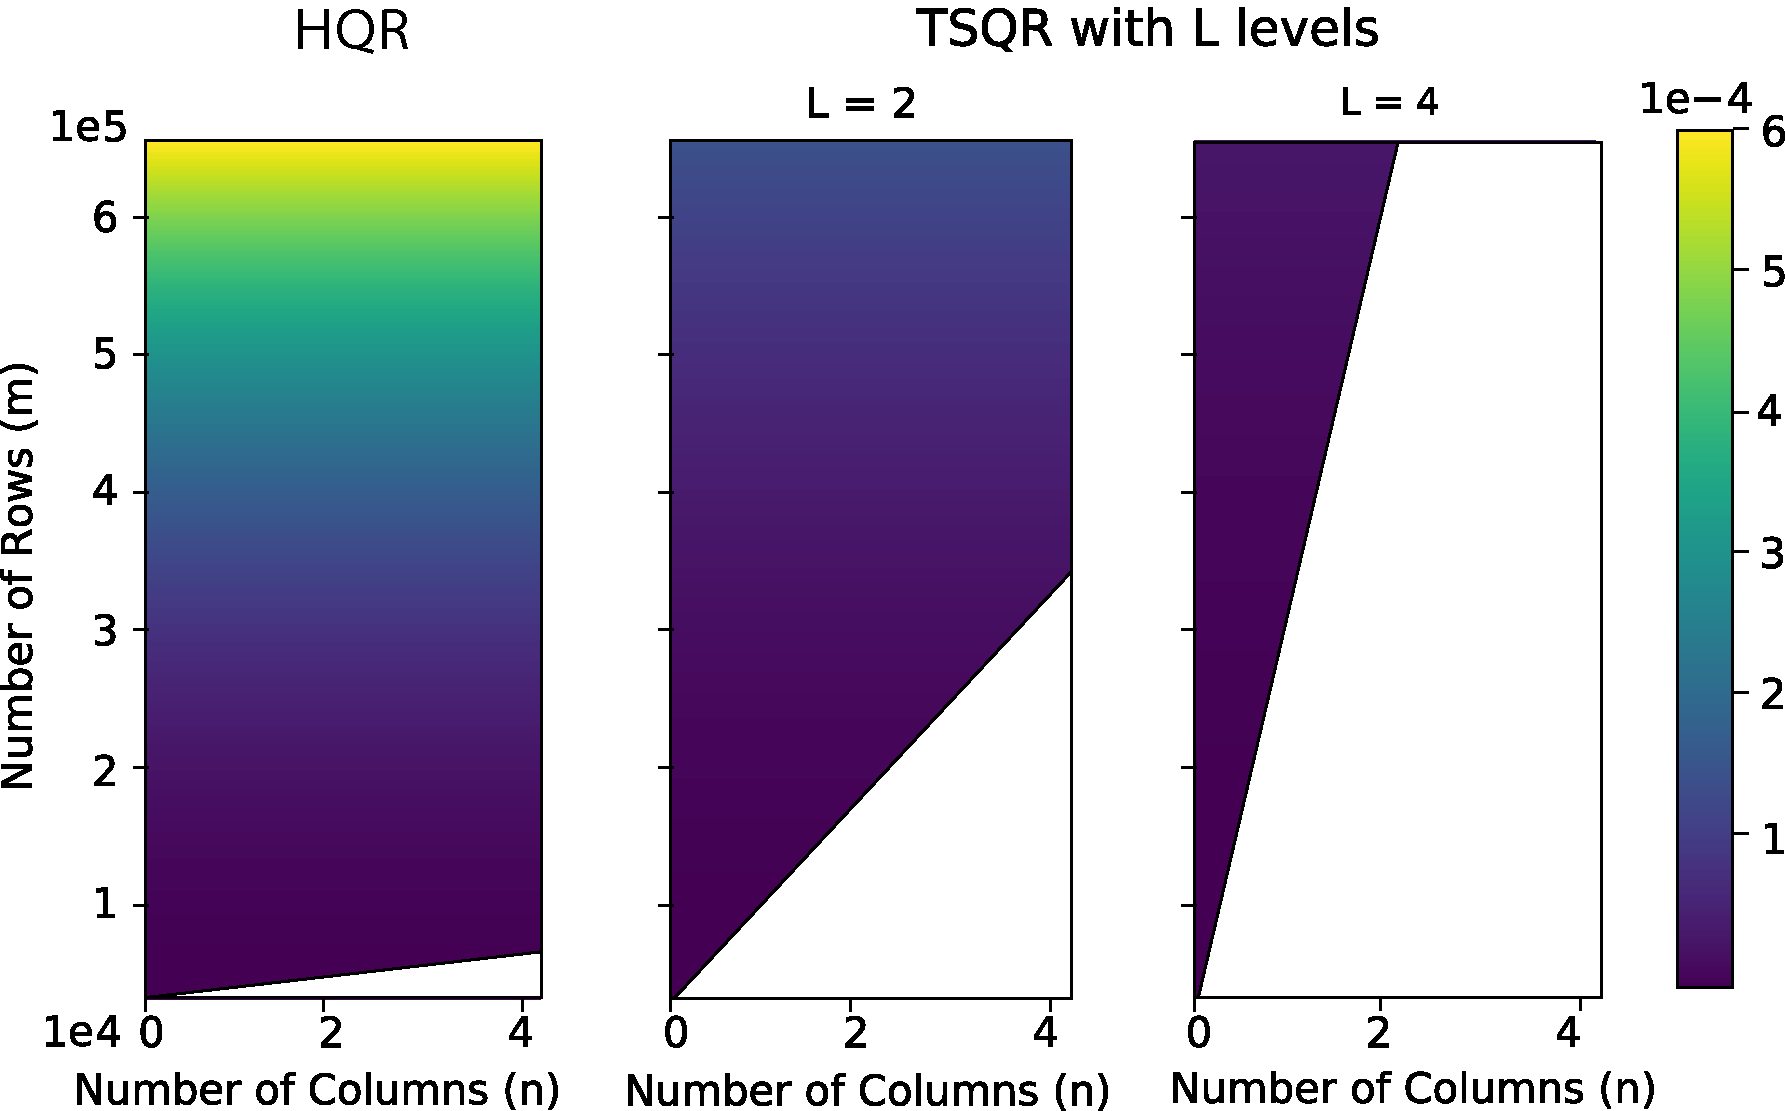
\includegraphics[width=0.45\textwidth]{./figures/paramspace.png}
    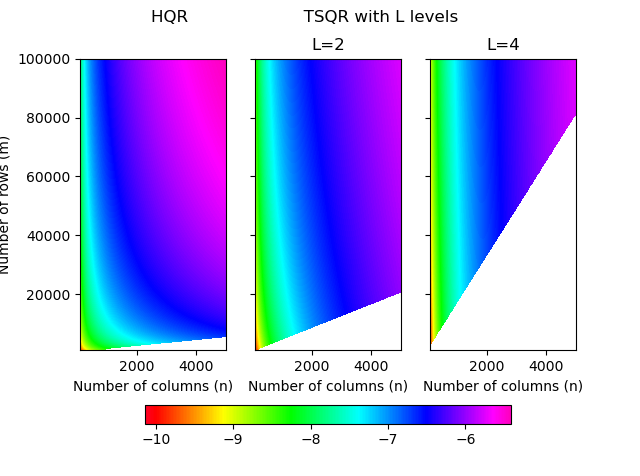
\includegraphics[width=0.45\textwidth]{./paramspace2.png}
    \caption{\label{fig:Fig1}Left plot: Old; Right plot: New}
    \vspace{-10pt}
\end{figure} 

    \item {\it Section 4: I think the paper would read better by interchanging sections 4.1 and 4.2. The bounds of section 4.2 are weaker, and adding them after section 4.1 therefore seems artificial and unnecessary. Instead, giving first the bounds for the more general MP setting 2.3 would allow to present the bFMA/TensorCore setting as a further improvement, which would neatly emphasize the accuracy benefits brought by this type of hardware.}\\
    {\bf We have made this change to the manuscript. However, this change is not reflected in the diff.pdf I provided to aid with this submission.}
    \item {\it Equation (4.5): $\gamma_{p/4}^{(fp32)}$ should be replaced by $\gamma_p^{(fp32)}$. In an early preprint version of \cite{Blanchard2020}, the former was indeed given under the assumption that NVIDIA tensor cores implement a “true FMA”, that is, that in (4.4) the additions in the $4\times 4$ product AB are done in full precision. However this is not the case, the additions are performed in fp32, and so there are still p rounding errors that accumulate in a general product of inner dimension p, as indicated in the published version of \cite{Blanchard2020} (cf. [1, Thm 3.1]). Fortunately I do not think this impacts the analysis of this paper beyond equation (4.5).}\\
    {\bf The change has been made to the manuscript.}
    \item {\it The discussion on L684–691 is overall OK, although I feel that there are two points that could be better emphasized.}
    \begin{itemize}
        \item First, the sentence “However, as $r$ grows large. . . ” makes it seems as if $r$ should be taken as small as possible for performance, but of course this is not the case since the factorization then also reduces to BLAS-2 operations. In practice, realistic values of $r$ probably range between $\cO(10)$ and $\cO(100)$, depending on hardware, and not discussing double partitioning strategies. So it is entirely possible that the optimal value of $r$for performance is already quite large enough so that the accuracy is satisfying.
        \item Second, for a fixed $r$, (4.11) shows that the loss of accuracy becomes less and less significand as m increases and so asymptotically, regardless of the practical value of $r$, the accuracy eventually will be satisfying. I feel this should be mentioned.
    \end{itemize}
    {\bf We have discussed the above two points in this part of the discussion.}
    \item I suggest adding a Table at the end of section 4 or beginning of section 5 sum- marizing the bounds obtained for each of the 9 algorithms: \{H,B,TS\}QR and mp\{H,B,TS\}QR\{2,3\}. It would really be useful to have such a Table, for other ar- ticles to refer to, and as reference when comparing with the numerical experiments of section 5.\\
    {\bf The table has been added.}
    \item Figure 2, left plot: I suggest fixing $r$ to a constant rather than $n/4$, which I think is more realistic. Also, have the authors checked what the plots look like for fixed $n$ rather than $n = m/4$ ? The bounds suggest n should not play a significant role in the relative accuracy of the MP block algorithms vs. the uniform precision ones, but it might be worth checking.\\
    {\bf We fixed $n=250$ (to accomodate for $L=2$ for TSQR) and $r=63$. Keeping $n$ small reduced the errors for all of the BLAS-2 methods, so we updated the figure to this version. The high precision and BLAS-3 methods remained pretty much the same. }
    \item Figure 2, right plot: the chosen m is a bit small, would it be worth giving the errors for a larger $m$ (which would probably lead to the MP and uniform algorithms to be closer in accuracy) ?\\
    {\bf We had tried increasing $m$, but it looked that the matrices needed to be significantly larger to grow sufficiently closer together. Figures with larger matrix sizes are shown in \cref{fig:Fig2}. Notably, the rightmost plot show the {\tt mpBQR3} orthogonality error to drop below the unit round-off for fp16. Below are similar figure with larger matrix sizes. Our goal with this figure was to show that the errors do behave in the same trend as the error bounds suggest and therefore we have kept the figure.}
    \begin{figure}[h!]
        \centering
        \vspace{-10pt}
        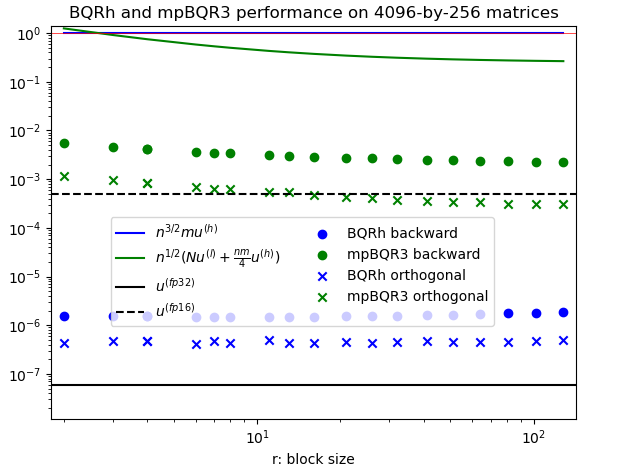
\includegraphics[width=0.32\textwidth]{./figures/12-08.png}
        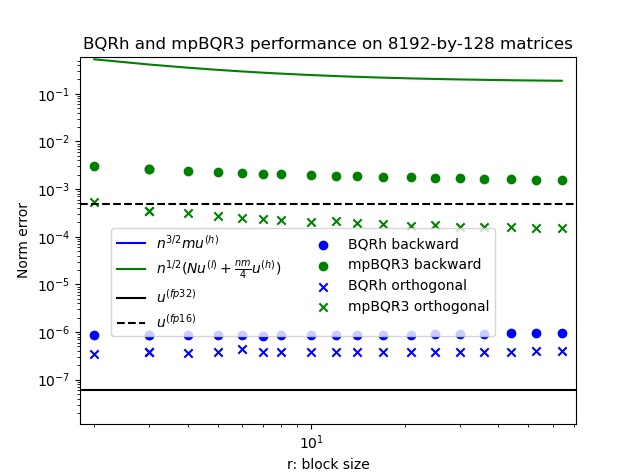
\includegraphics[width=0.32\textwidth]{./figures/13-07.png}
        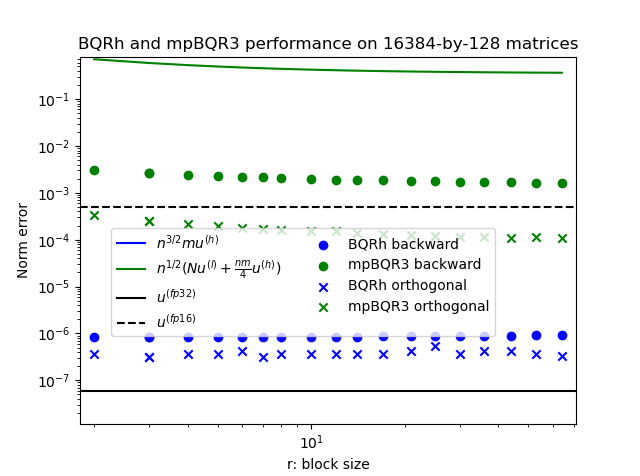
\includegraphics[width=0.32\textwidth]{./figures/14-07.png}
        \caption{\label{fig:Fig2} Left: Old figure; Middle: Larger matrices; Right: Largest matrices.}
        \vspace{-10pt}
    \end{figure} 
\end{enumerate}
\pagebreak
\textbf{Stylistic suggestions, typos, and other very minor things:}
\begin{enumerate}
    \item {\it Everywhere: a HH $\rightarrow$ an HH.}\\
    {\bf Done.}
    \item {\it L44: columns $\rightarrow$ rows.}\\
    {\bf Done.}
    \item {\it L120–123: the behavior of the error depending on the data distribution has been explained in the recent preprint \cite{HighamMary2020}, which could be referenced here.}
    \item {\it L157: Assumption 2.3 $\rightarrow$ MP Setting 2.3.}\\
    {\bf Done.}
    \item {\it L175: the notation $x^{(l)}$, $y^{(l)}$ is introduced but does not seem to be used in the
subsequent analysis.}\\
	{\bf This notation was dropped for this paragraph. }
    \item {\it L233–236: I did not fully understand these two sentences. I think the authors are saying that computations introduce error terms of the form (2.9) while castdowns introduce error terms of the form (2.10). Perhaps consider clarifying or removing these two sentences.}\\
    {\bf These sentences have been rephrased.}
    \item {\it L255, L261, L382, L384, L733: zeros out $\rightarrow$ zeroes out.}\\
    {\bf Done.}
    \item {\it L288: remove “between”.}\\
    {\bf Done.}
    \item {\it L294: (3.7) show $\rightarrow$ (3.7) to show ?}\\
    {\bf Done.}
    \item {\it L295: calculating of $\|x\|\rightarrow$ remove ``of''.}\\
    {\bf Done.}
    \item {\it L316, L317, L319: I suggest rewriting $v^{\top}xv$ either as $vv^{\top} x$ or $(v^{\top} x)v$.}\\
    {\bf Done.}
    \item {\it (3.13): $\Delta y \rightarrow \Delta x$.}\\
    {\bf I think this should be $\Delta y$ as is stated in (3.10).}
    \item {\it L375: constants, $\beta \rightarrow$ missing space.}\\
    {\bf Space added.}
    \item {\it L385: $k+1^{st} \rightarrow (k+1)^{th}$, idem at L420.}\\
    {\bf Fixed.}
    \item {\it L397, L617: TensorCore $\rightarrow$ TensorCores ?}\\
    {\bf Fixed.}
    \item {\it L399: negligble $\rightarrow$ negligible.}\\
    {\bf Fixed.}
    \item {\it L761: “the inner product mixed precision setting yields higher error bounds”: specify than what (add a reference to Thm. 3.4 ?)}\\
    {\bf Reference added.}
    \item {\it L762: I suggest adding a sentence of the form ``Before commenting on the significance of Theorem 4.1, we show that the same bounds hold for the BQR variant''. Otherwise section 4.2.1 ends a little abruptly and without any analysis of Thm 4.1 (which is in fact to be found later, L775–L783). In fact, perhaps consider merging sections 4.2.1 and 4.2.2 since the analysis and bounds are essentially the same?}\\
    {\bf The sentence has been added to better bridge the two sections, but they have been left as two distinct sections.}
    \item {\it L798: what are d1 and d2 here?}\\
    {\bf Oops, an artifact from the first submission had survived! This has been reworded.}
    \item {\it Sections 4.1.2 and 4.2.3: I suggest writing consistently either $2Ln + m2^{-L}$ (as in
section 4.1.2) or $m2^{-L} + 2Ln$ (as in section 4.2.3).}\\
    {\bf Done.}
    \item {\it L885: analysis that accurately bound $\rightarrow$ change to ``analyses'' or ``bounds''.}\\
    {\bf Done.}
    \item {\it Reference [5] has now appeared: cf. [1].} \\
    {\bf The reference has been updated.}
\end{enumerate}

\bibliographystyle{siamplain}%ieeetr
\bibliography{../../../../../library.bib,../../../../../sans_library.bib,./report.bib}

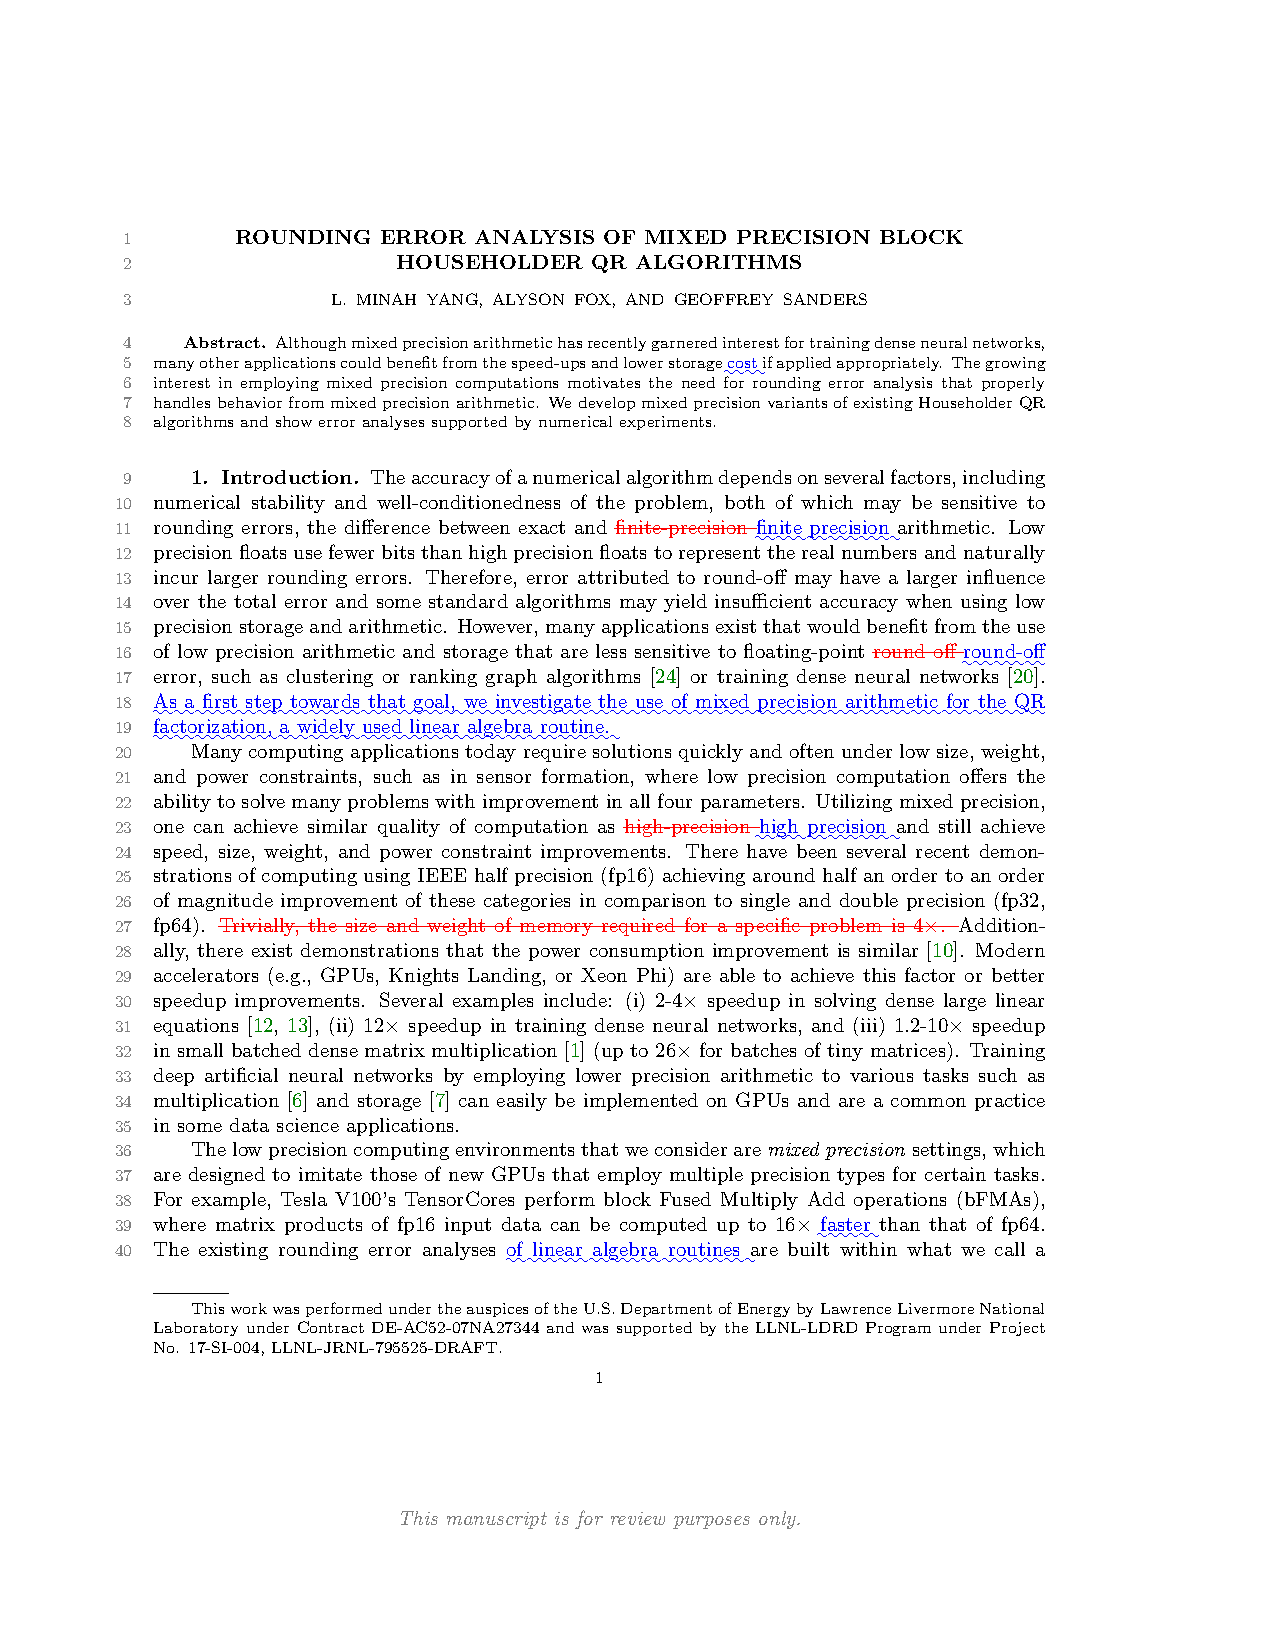
\includepdf[pages=-]{diff.pdf}
\end{document}